\section{Introduction}
The diffusion models (DMs) are powerful generative models that have demonstrated great performance \cite{ho2020denoising, song2020denoising, song2020score, dhariwal2021diffusion, nichol2021improved}. 
DMs have shown impressive applications, including text-to-image synthesis \cite{ramesh2022hierarchical, rombach2022high, balaji2022ediffi, nichol2021glide}, inverse problems \cite{lugmayr2022repaint, chung2022improving, lugmayr2022repaint}, and image editing \cite{hertz2022prompt, tumanyan2022plug, parmar2023zero, mokady2022null}.

% Diffusion models (DMs) are highly powerful generative models that have shown great performance \cite{ho2020denoising,song2020denoising,song2020score,dhariwal2021diffusion,nichol2021improved}.
% \yh{Instead of understanding the semantic structure of latent space itself,} 
% To control the generative process,
% existing methods have introduced conditional DMs, especially for text-to-image synthesis \cite{ramesh2022hierarchical,rombach2022high,balaji2022ediffi,nichol2021glide}, or mixing the latent variables $\vx_t$ of different sampling processes \cite{choi2021ilvr,meng2021sdedit,avrahami2022blended,liew2022magicmix,kawar2022imagic,avrahami2022spatext}.

Despite their achievements, the research community still lacks a clear understanding of the semantic structure of DMs and how it is represented in the resulting images.
This can be attributed to the fact that the latent variable of DM, $\vx{}_t$, consists primarily of noised images.
% images disrupted by adding Gaussian noise.
As a consequence, it is not reasonable to expect any significant semantic structure in the latent space $\vx{}_t \in \mathcal{X}$.

% Despite their success, the research community still lacks a clear understanding of what the latent variables or intermediate features of the models are embedded or how they are reflected in the resulting images. 
% \yh{
% We attribute it to the characteristic of the latent variable of DMs $\vx{}_t$ which is mere disruption of original images. As a result, it is not reasonable to expect any meaningful semantic structure in the latent space $\vx{}_t \in \mathcal{X}$.
% We attribute it to the characteristic of the latent variable of DMs $\vx{}_t$ which is disrupted image with gaussian noise. Therefore, we cannot expect any semantic structure in the latent space $\vx{}_t \in \mathcal{X}$.
% }

% \mingi{We attribute it to the characteristic iterative process of the DMs which involves a sequence of noisy images and subtle noises, i.e., the embeddings are not directly connected to the final images.}
% \mingi{Therefore, although we can regard the diffused noisy images, latent variables of DMs, as the latent space of DMs, the semantic adjustment method in the latent space has not been revealed.} 
% In contrast, arithmetic operations in the latent space of generative adversarial networks (GANs) lead to semantic changes in the resulting images \cite{goodfellow2020generative}. This property has been one of the key factors in developing GANs for real-world applications. We suppose that a better understanding of the latent space of DMs will boost similar development.

\begin{figure}[!t]
    \centering
    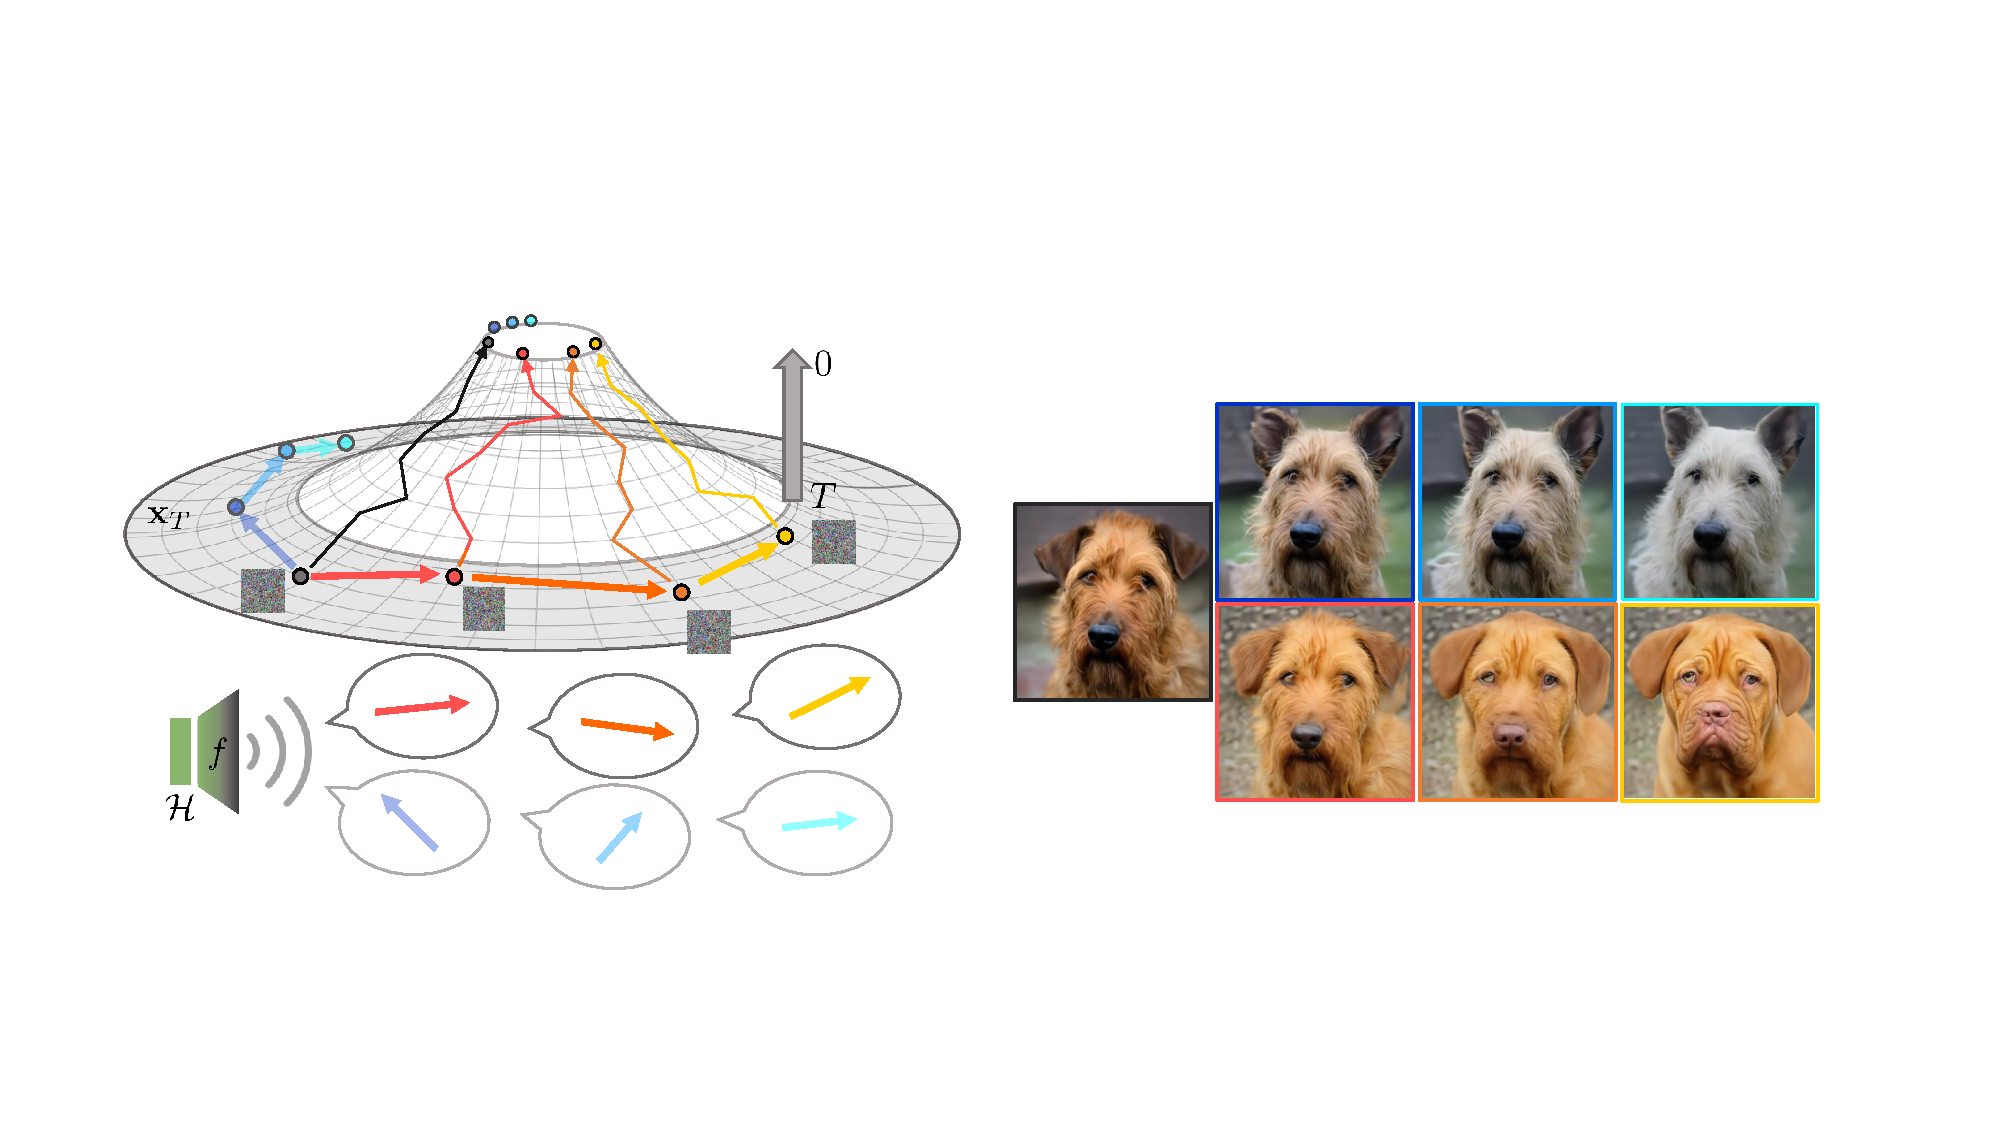
\includegraphics[width=0.9\linewidth]{./figure/teaser.pdf}
    \caption{\textbf{Conceptual illustration of our method.} 
    We find semantic directions in the latent space $\vx_t$ in an unsupervised fashion relying on Riemannian geometry between $\vx_t$ and $\vh_t$. $\mathcal{H}$ denotes the bottleneck layer and $f$ indicates the frozen encoder of a U-Net. 
    The found directions manipulate the semantics of the resulting images.
    }
    \vspace{-1em}
    \label{fig:main_concept}
\end{figure}

% \citet{kwon2022diffusion} adopt the intermediate feature space of the diffusion kernel as a semantic latent space, namely \ehspace{}, paired with a designated asymmetric sampling process. They revealed the local linearity of \ehspace{}.
% % , adding to our understanding of the latent space of DMs.
% However, they do not directly deal with the latent variables $\vx_t$ but rely only on a proxy, $\mathbf{h}$. 
% % Furthermore, they require external supervision such as Contrastive Language-Image Pretraining (CLIP) to find editable directions. \cite{radford2021learning}
% Since latent space \exspace{} is a sparse manifold, it is certainly not easy to do meaningful editing in it. However, \ehspace{} is clearly the codomain of \exspace{}, and the fact that we can find a meaningful semantic direction in \ehspace{} means that we can define semantic subspace in \exspace{} as well.

Fortunately, \citet{kwon2022diffusion} employed the intermediate feature space of the diffusion kernel, referred to as \ehspace{}, as a semantic latent space. 
% They pair this with an asymmetric sampling process and
They demonstrated that \ehspace{} possesses a linear semantic structure.
% However, they rely solely on a proxy, $\mathbf{h}$, and do not directly deal with the latent variables $\vx_t$. 
% Furthermore, due to Kwon et al.'s modification of the internal feature of UNet, particularly where skip connections exist, there is no guarantee that significant changes will result in output quality. It is worth noting that the latent space \exspace{} is a sparse manifold, which makes meaningful editing within it challenging. Nevertheless, since \ehspace{} is clearly the codomain of \exspace{}, and given the fact that a meaningful semantic direction can be found in \ehspace{}, we can also define a semantic subspace in \exspace{}.
{
    After the work of \citet{kwon2022diffusion}, there have been several analyses of the DM's feature space. These include investigations into the attention map and cross-attention map, which have been used for image editing \cite{hertz2022prompt, tumanyan2022plug, parmar2023zero} or improving sample quality \cite{chefer2023attend}. Furthermore, these discoveries can be applied to downstream tasks such as segmentation using the feature space \cite{ma2023diffusionseg, xu2023open}.
    % Following the work of Kwon et al., there have been several analyses of DM's feature space. 
    % For instance, there are studies that examine the attention map and cross-attention map, utilizing them for tasks such as image editing or improving sample quality \cite{hertz2022prompt, tumanyan2022plug, parmar2023zero, chefer2023attend}. 
    % Additionally, these discoveries can be utilized for downstream tasks, including segmentation using the feature space \cite{ma2023diffusionseg, xu2023open}.
}

% \mingi{
% \citet{kwon2022diffusion} utilize the intermediate feature space of the diffusion kernel, which they refer to as \ehspace{}, as a semantic latent space. They pair this with an asymmetric sampling process and demonstrate the local linearity of \ehspace{}. However, they rely solely on a proxy, $\mathbf{h}$, and do not directly deal with the latent variables $\vx_t$. Furthermore, due to Kwon et al.'s modification of the internal feature of UNet, particularly where skip connections exist, there is no guarantee that significant changes will result in output quality. It is worth noting that the latent space \exspace{} is a sparse manifold, which makes meaningful editing within it challenging. Nevertheless, since \ehspace{} is clearly the codomain of \exspace{}, and given the fact that a meaningful semantic direction can be found in \ehspace{}, we can also define a semantic subspace in \exspace{}.
% }

Although there has been a thorough exploration of the feature space, the latent space \exspace{} remains unexplored, even though it plays a crucial role in understanding DMs.
In this paper, we aim to analyze \exspace{} in conjunction with its corresponding representation \ehspace{}, by introducing a local semantic structure to \exspace{} using the concept of a {\it pullback metric} in Riemannian geometry. 
The contributions of our paper are as follows: 
% The pullback metric is a powerful tool in differential geometry that enables the study of the geometry of one manifold in terms of another manifold. 
% By analyzing the discovered semantic structure, we are able to shed light on the intriguing properties of DMs.

% \yh{ By investigating the semantic structure of \exspace{} in conjunction with its corresponding representation space \ehspace{}, we can gain insights into the signals used in latent variables and how they are influenced by other parameters such as timestep or text prompt. Moreover, we can also utilize the discovered semantic basis for the purpose of editing real images to achieve specific properties or characteristics. }
% This enables us to generate new samples with desired characteristics by manipulating the values of the latent variables. 
% By visualizing the latent space, we can gain a better understanding of how the model is learning and how it represents the data

% \mingi{we can manipulate the values of the latent variables to generate new samples with specific properties or characteristics. Visualizing the latent space can help us understand how the model is learning and how it represents the data. }

% \yh{In this paper, we aims to discover semantic structure, i.e. semantic subspace and semantic basis, of latent space and feature space, namely \exspace{} and \ehspace{}, in \emph{pretrained and frozen} DMs by utilizing the Riemannian geometry. By analyzing the discovered semantic structure, we are able to shed light on intriguing properties of DMs.} 

First, we discover the local semantic basis and their corresponding local tangent basis within \exspace{} and \ehspace{}, respectively. 
The local basis is obtained through singular value decomposition (SVD) of the Jacobian of the mapping from \exspace{} to \ehspace{}.
% , which is the intermediate feature space of the U-Net model. 
To verify the discovered local semantic basis, we demonstrate their capability to edit real images in a semantically meaningful way. 
\yh{ Moreover, based on the observation that multiple samples exhibit comparable local semantic structures, we are able to create a global semantic basis using the \frechet{} mean. } It follows the course of generative adversarial networks: extending per-sample editing directions \cite{ramesh2018spectral,patashnik2021styleclip,abdal2021styleflow,shen2021closed} to global editing directions \cite{harkonen2020ganspace,shen2021closed,yuksel2021latentclr}.

% \yh{
% Based on the observation that multiple samples exhibit comparable local semantic structures, we create a global semantic basis using the \frechet{} mean.
% It removes the cumbersome process of checking the semantic meaning of basis sample-by-sample and allows general controllability.
% It follows the course of generative adversarial networks: extending per-sample editing directions \cite{ramesh2018spectral,patashnik2021styleclip,abdal2021styleflow,shen2021closed} to global editing directions \cite{harkonen2020ganspace,shen2021closed,yuksel2021latentclr}.
% }

Secondly, we investigated how the semantic structure changes over time and identified two trends.
\textcircled{\raisebox{-0.9pt}{1}} The frequency domain of the local semantic basis shifted from low-frequency to high-frequency detail as image generation progressed. 
While this trend has been indirectly observed in previous studies by \citet{choi2022perception}, we provide explicit confirmation through power spectral density analysis.
\textcircled{\raisebox{-0.9pt}{2}} We compared the local semantic basis over time and found that there are two major regimes in the denoising process. \todo{Something more information about clusters.}
% gDDIM 의 denoising process 를 나누는 기준을 떠올리게 한다. 
% TODO
% 이 관찰으로부터 유사한 semantic structure 를 갖는 구간을 clustering 하고, 각 cluster 에서 redundant 하지 않은 timestep scheduling 을 제안하고 sampling quality 를 개선했다.

Finally, we investigated how the prompts affect the semantic structure of text-to-image DMs and obtained two key insights.
\textcircled{\raisebox{-0.9pt}{1}} We observed that similar prompts result in similar semantic structures. Specifically, we found a positive correlation between the similarity of the prompt in the CLIP model and the similarity of local tangent subspaces.
\textcircled{\raisebox{-0.9pt}{2}} We discovered that the effect of text on the local tangent space became weaker and weaker as the denoising process progresses, specifically when $t<0.7T$.

\yh{TODO : Intro 마무리 요약 멘트}

% In the experiments, we demonstrate that the directions found in an unsupervised manner indeed lead to semantic changes in the images. 
% We note that discovering the editing directions in the latent variables of diffusion models has not been tackled.
% \mingi{}
% Furthermore, we provide thorough quantitative and qualitative analyses on the aforementioned properties. Our method even works on stable diffusion \cite{rombach2022high}.
